\section{Исследование эффективности применения реализованного программного модуля}

Исследуем эффективность предлагаемой оптимизации. Для этого рассмотрим задачи, описанные в разделе \ref{sec_problem}.
Ключевым параметром, который должна затрагивать оптимизация, является время, затраченное на десериализацию protobuf-сообщения.
Также с помощью утилиты \textit{perf} и инструмента визуализации \textit{flamegraph.pl} сравним процент времени, уходящего на распаковку сообщений, по отношению ко всему времени работы алгоритма.

\subsection{Задача фильтрации списка массивных сообщений по легковесному полю}

Рассмотрим задачу, описанную в подразделе \ref{sec_problem:sec:problem1}.
В целях замера производительности опишем тестовое protobuf-сообщение, представленное в листинге \ref{sec_research:code:problem1_proto}.

\noindent\begin{minipage}{\linewidth}
\begin{lstlisting}[style=CodeListing, caption={Тестовое protobuf-сообщение}, label=sec_research:code:problem1_proto]
syntax = "proto3";

message TBigProto {

    message TBigInternalMessage {
        repeated string StringsArr = 1;
        repeated int32 IntsArr = 2;
    }

    int32 Timestamp = 1;

    TBigInternalMessage BigInternal1 = 2 [lazy_pack = true];
    TBigInternalMessage BigInternal2 = 3 [lazy_pack = true];
    TBigInternalMessage BigInternal3 = 4 [lazy_pack = true];
}
\end{lstlisting}
\end{minipage}

Благодаря полям \textit{StringsArr} и \textit{IntsArr}, поля \textit{BigInternal1}, \textit{BigInternal2} и \textit{BigInternal3} могут иметь достаточно большой вес.
Сгенерируем тестовые данные. Для этого опишем вспомогательные функции. В листинге \ref{sec_research:code:problem1_generate_big_string} представлена функция \textit{GenerateBigString}, создающая строку, состоящую из \textit{len} случайных строчных латинских символов.

\noindent\begin{minipage}{\linewidth}
\begin{lstlisting}[style=CodeListing, caption={Функция GenerateBigString}, label=sec_research:code:problem1_generate_big_string]
std::string GenerateBigString(size_t len) {
    std::string res(len, 'a');
    for (size_t i = 0; i < len; i++) {
        res[i] = 'a' + (rand() % 26);
    }

    return res;
}
\end{lstlisting}
\end{minipage}

В листинге \ref{sec_research:code:problem1_generate_big_internal_message} представлена функция \textit{GenerateBigInternalMessage}, создающая protobuf-сообщение \textit{TBigProto::TBigInternalMessage}, содержащее массив \textit{StringsArr}, состоящий из \textit{numOfStrings} случайных строк длины \textit{lenOfString} случайных строчных латинских символов, а также массив \textit{IntsArr}, содержащий \textit{numOfInts} случайных чисел от 0 до 500.

\noindent\begin{minipage}{\linewidth}
\begin{lstlisting}[style=CodeListing, caption={Функция GenerateBigInternalMessage}, label=sec_research:code:problem1_generate_big_internal_message]
TBigProto::TBigInternalMessage GenBigInternalMessage(size_t numOfStrings, size_t lenOfString, size_t numOfInts) {
    TBigProto::TBigInternalMessage result;
    for (size_t i = 0; i < numOfStrings; i++) {
        result.MutableStringsArr()->Add(GenerateBigString(lenOfString));
    }

    for (size_t i = 0; i < numOfInts; i++) {
        result.MutableIntsArr()->Add(rand() % 500);
    }

    return result;
}
\end{lstlisting}
\end{minipage}

В листинге \ref{sec_research:code:problem1_build_test_protos} представлена функция \textit{BuildTestProtos}, которая генерирует запрошенное количество protobuf-сообщений типа \textit{TBigProto} и записывает бинарное представление каждого из них в отдельный файл.

\noindent\begin{minipage}{\linewidth}
\begin{lstlisting}[style=CodeListing, caption={Функция BuildTestProtos}, label=sec_research:code:problem1_build_test_protos]
void BuildTestProtos(size_t n, size_t numOfStrings, size_t lenOfString, size_t numOfInts) {
    for (size_t i = 0; i < n; i++) {
        std::ofstream out(TStringBuilder{} << "./serialized/" << i << ".bin");
        TBigProto bigProto;
        bigProto.SetTimestamp(i);
        bigProto.MutablebigInternal1()->CopyFrom(GenBigInternalMessage(numOfStrings, lenOfString, numOfInts));
        bigProto.MutablebigInternal2()->CopyFrom(GenBigInternalMessage(numOfStrings, lenOfString, numOfInts));
        bigProto.MutablebigInternal3()->CopyFrom(GenBigInternalMessage(numOfStrings, lenOfString, numOfInts));
        out << bigProto.SerializeAsString();
    }
}
\end{lstlisting}
\end{minipage}

С помощью функции \textit{BuildTestProtos} были сгенерированы 100 сериализованных protobuf-сообщений. Вес каждого из них в сериализованном виде составил 3.5 мегабайта.
Рассмотрим функцию для замера производительности \textit{Measure}, представленную в листинге \ref{sec_research:code:problem1_measure}.
Она занимается поочерёдным открытием файлов с сериализованными сообщениями,
их десериализацией и проверкой поля \textit{Timestamp}. Если оно попадает в нужные границы, производится доступ к первому элементу массива \textit{IntsArr} поля \textit{BigInternal1}, что в случае <<ленивой>> десериализации должно вызвать распаковку поля \textit{BigInternal1}.

\noindent\begin{minipage}{\linewidth}
\begin{lstlisting}[style=CodeListing, caption={Функция Measure}, label=sec_research:code:problem1_measure]
void Measure() {
    for (size_t i = 0; i < 100; i++) {
        std::ifstream in(TStringBuilder{} << "./serialized/" << i << ".bin");
        std::string str(std::istreambuf_iterator<char>{in}, {});
        TString encoded(str);
        TBigProto bigProto;
        Cerr << "---------------\n";
        auto start = TInstant::Now();
        Y_ENSURE(bigProto.ParseFromString(encoded));
        Cerr << "Deserialization took " << (TInstant::Now() - start).MicroSeconds() << "mcs;\n";
        start = TInstant::Now();
        if (bigProto.GetTimestamp() > 25 && bigProto.GetTimestamp() < 50) {
            auto x = bigProto.GetbigInternal1().GetIntsArr().Get(0);
            Cerr << "Found good item. First item of IntsArr in BigInternal1: " << x << "\n";
        }
        Cerr << "Check (and maybe access) took " << (TInstant::Now() - start).MicroSeconds() << "mcs\n";
    }
}
\end{lstlisting}
\end{minipage}

На рисунке \ref{fig:problem1_vanilla_timings_false_cond} представлена часть замеров в случае неизменённого \textit{protoc}. 
Данные сообщения не подходили под условия фильтрации, и в этом случае было затрачено около 26 миллисекунд на десериализацию сообщения и ничтожно малое время на проверку условия фильтрации.

\begin{figure}[ht]
    \centering
    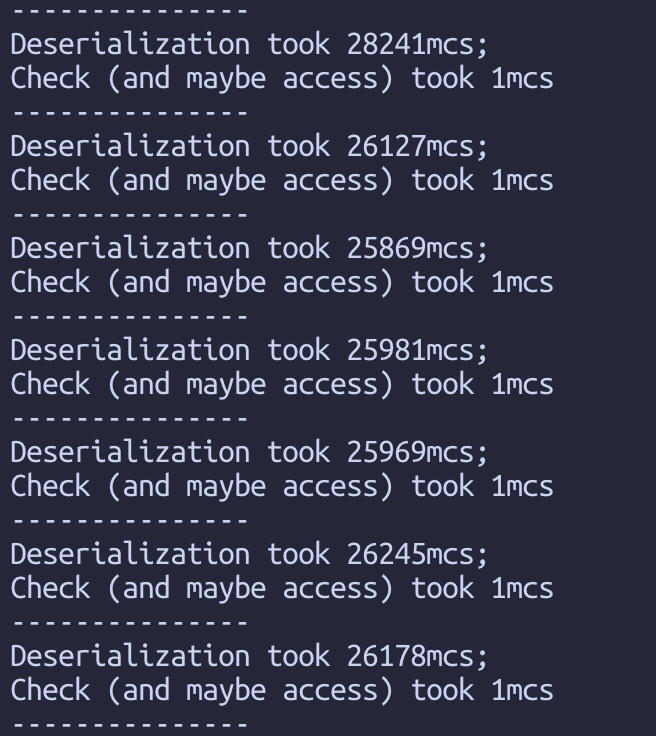
\includegraphics[width=0.60\linewidth]{\commonSecPathPrefix/sec_research_results_attachments/problem1_vanilla_timings_false_cond.png}
    \caption{Время десериализации одного сообщения в случае неизменённого protoc и невыполнения условия}
    \label{fig:problem1_vanilla_timings_false_cond}
\end{figure}

На рисунке \ref{fig:problem1_vanilla_timings_true_cond} представлена часть замеров в случае неизменённого \textit{protoc}, однако данные сообщения подходили под условия фильтрации. В этом случае времязатраты практически не изменились.

\begin{figure}[ht]
    \centering
    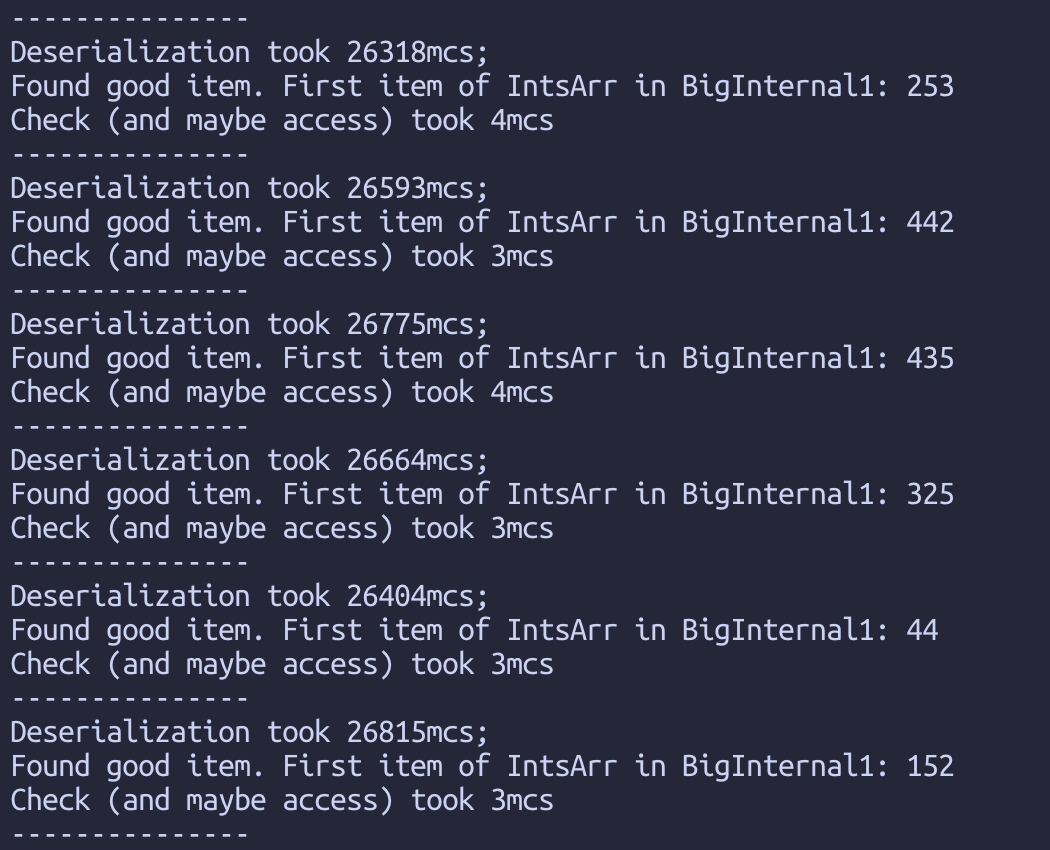
\includegraphics[width=0.60\linewidth]{\commonSecPathPrefix/sec_research_results_attachments/problem1_vanilla_timings_true_cond.png}
    \caption{Время десериализации одного сообщения в случае неизменённого protoc и выполнения условия}
    \label{fig:problem1_vanilla_timings_true_cond}
\end{figure}

Рассмотрим версию \textit{protoc} с интегрированным модулем <<ленивой>> десериализации.
На рисунке \ref{fig:problem1_patched_timings_false_cond} представлена часть замеров в случае, когда сообщения не подходили под условия фильтрации. На десериализацию затрачивается в 3 раза меньше времени ~--~ около 9 миллисекунд.

\begin{figure}[ht]
    \centering
    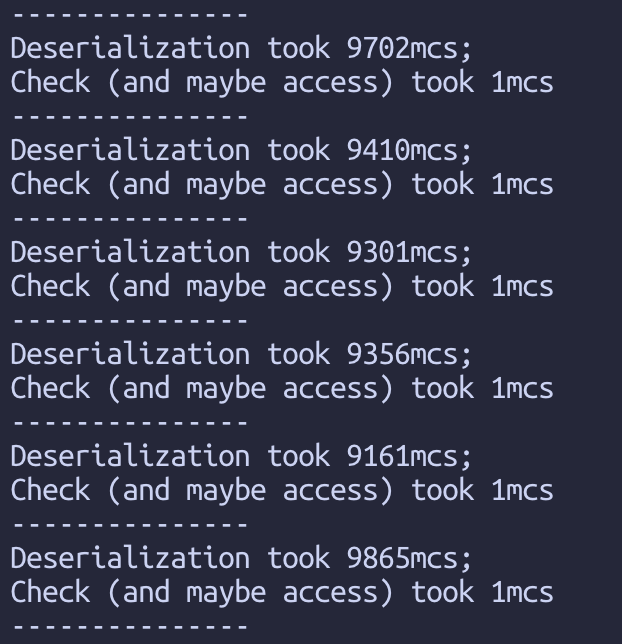
\includegraphics[width=0.60\linewidth]{\commonSecPathPrefix/sec_research_results_attachments/problem1_patched_timings_false_cond.png}
    \caption{Время десериализации одного сообщения в случае изменённого protoc и невыполнения условия}
    \label{fig:problem1_patched_timings_false_cond}
\end{figure}

На рисунке \ref{fig:problem1_patched_timings_true_cond} представлена часть замеров в случае, когда сообщения подходили под условия фильтрации. В этом случае времязатраты на первичную десериализацию остались прежними, однако доступ к <<ленивому>> полю породил ещё одну десериализацию, в среднем занимающую около 8 миллисекунд. 

\begin{figure}[ht]
    \centering
    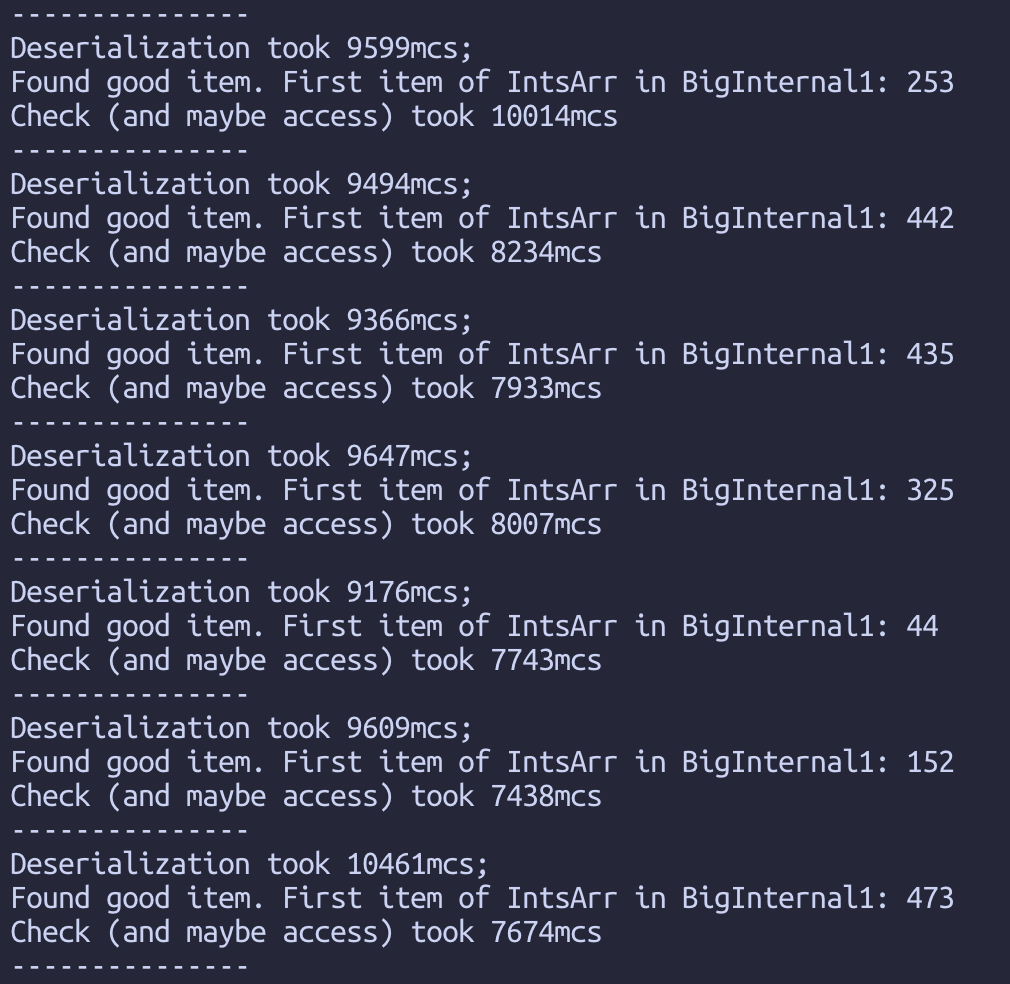
\includegraphics[width=0.60\linewidth]{\commonSecPathPrefix/sec_research_results_attachments/problem1_patched_timings_true_cond.png}
    \caption{Время десериализации одного сообщения в случае изменённого protoc и выполнении условия}
    \label{fig:problem1_patched_timings_true_cond}
\end{figure}

Построим флеймграфы для данных алгоритмов. В листинге \ref{sec_research:code:problem1_perf} представлена bash-инструкция, используемая для получения данных с помощью утилиты \textit{perf}.

\noindent\begin{minipage}{\linewidth}
\begin{lstlisting}[style=CodeListing, caption={bash-инструкция для сбора статистики утилитой perf}, label=sec_research:code:problem1_perf]
perf record \
    --call-graph dwarf,10000 \
    -F 250 \
    -g \
    --proc-map-timeout=10000 -- ./lazyproto_benchmark && \
perf script > out.perf
\end{lstlisting}
\end{minipage}

В листинге \ref{sec_research:code:problem1_fgraph} предсталена команда для формирования флеймграфа по полученной статистике от утилиты \textit{perf}.

\noindent\begin{minipage}{\linewidth}
\begin{lstlisting}[style=CodeListing, caption={bash-инструкция для сбора статистики утилитой perf}, label=sec_research:code:problem1_fgraph]
stackcollapse-perf.pl out.perf | \
c++filt > out.folded && \
flamegraph.pl out.folded > fgraph.svg
\end{lstlisting}
\end{minipage}

На рисунке \ref{fig:problem1_vanilla_fgraph} представлен флеймграф для алгоритма, использующего неизменённую версию \textit{protoc}. 
Работа с Protocol Buffers занимает 12.8\% от всего времени работы программы.

\begin{figure}[ht]
    \centering
    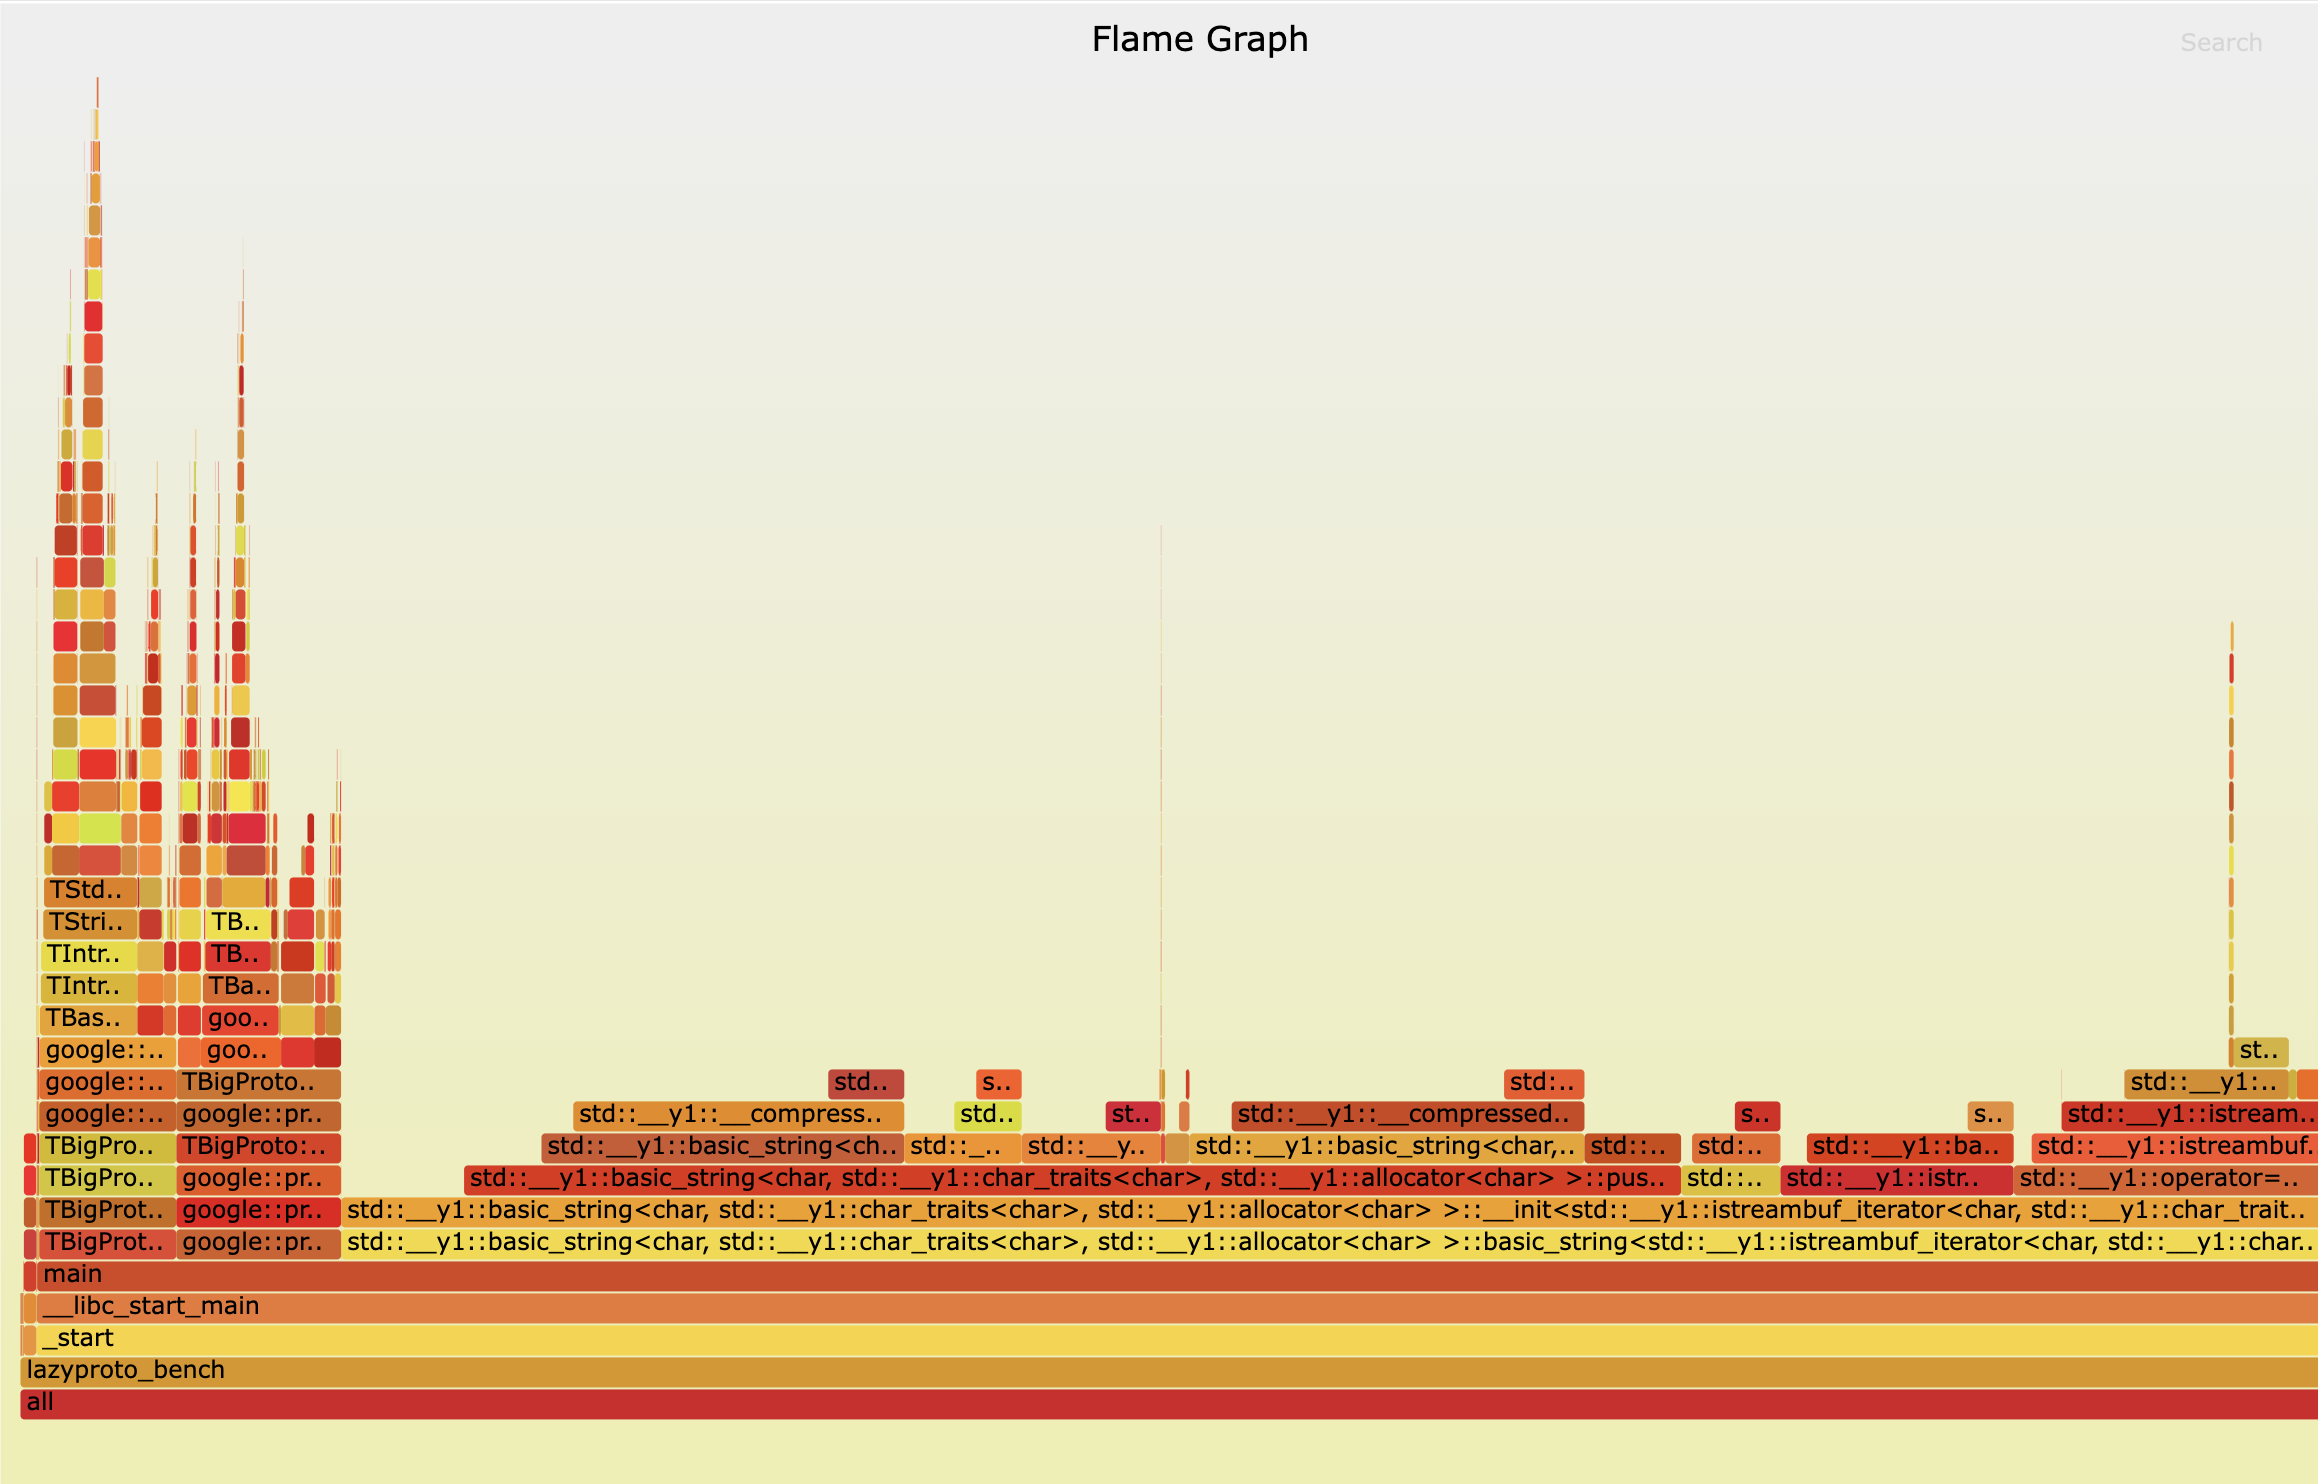
\includegraphics[width=0.70\linewidth]{\commonSecPathPrefix/sec_research_results_attachments/problem1_vanilla_fgraph.png}
    \caption{Флеймграф алгоритма с неизменённым protoc}
    \label{fig:problem1_vanilla_fgraph}
\end{figure}

На рисунке \ref{fig:problem1_patched_fgraph} представлен флеймграф для алгоритма, использующего версию \textit{protoc} с интегрированным модулем <<ленивой>> десериализации. 
Работа с Protocol Buffers занимает 2.4\% от всего времени работы программы.

\begin{figure}[ht]
    \centering
    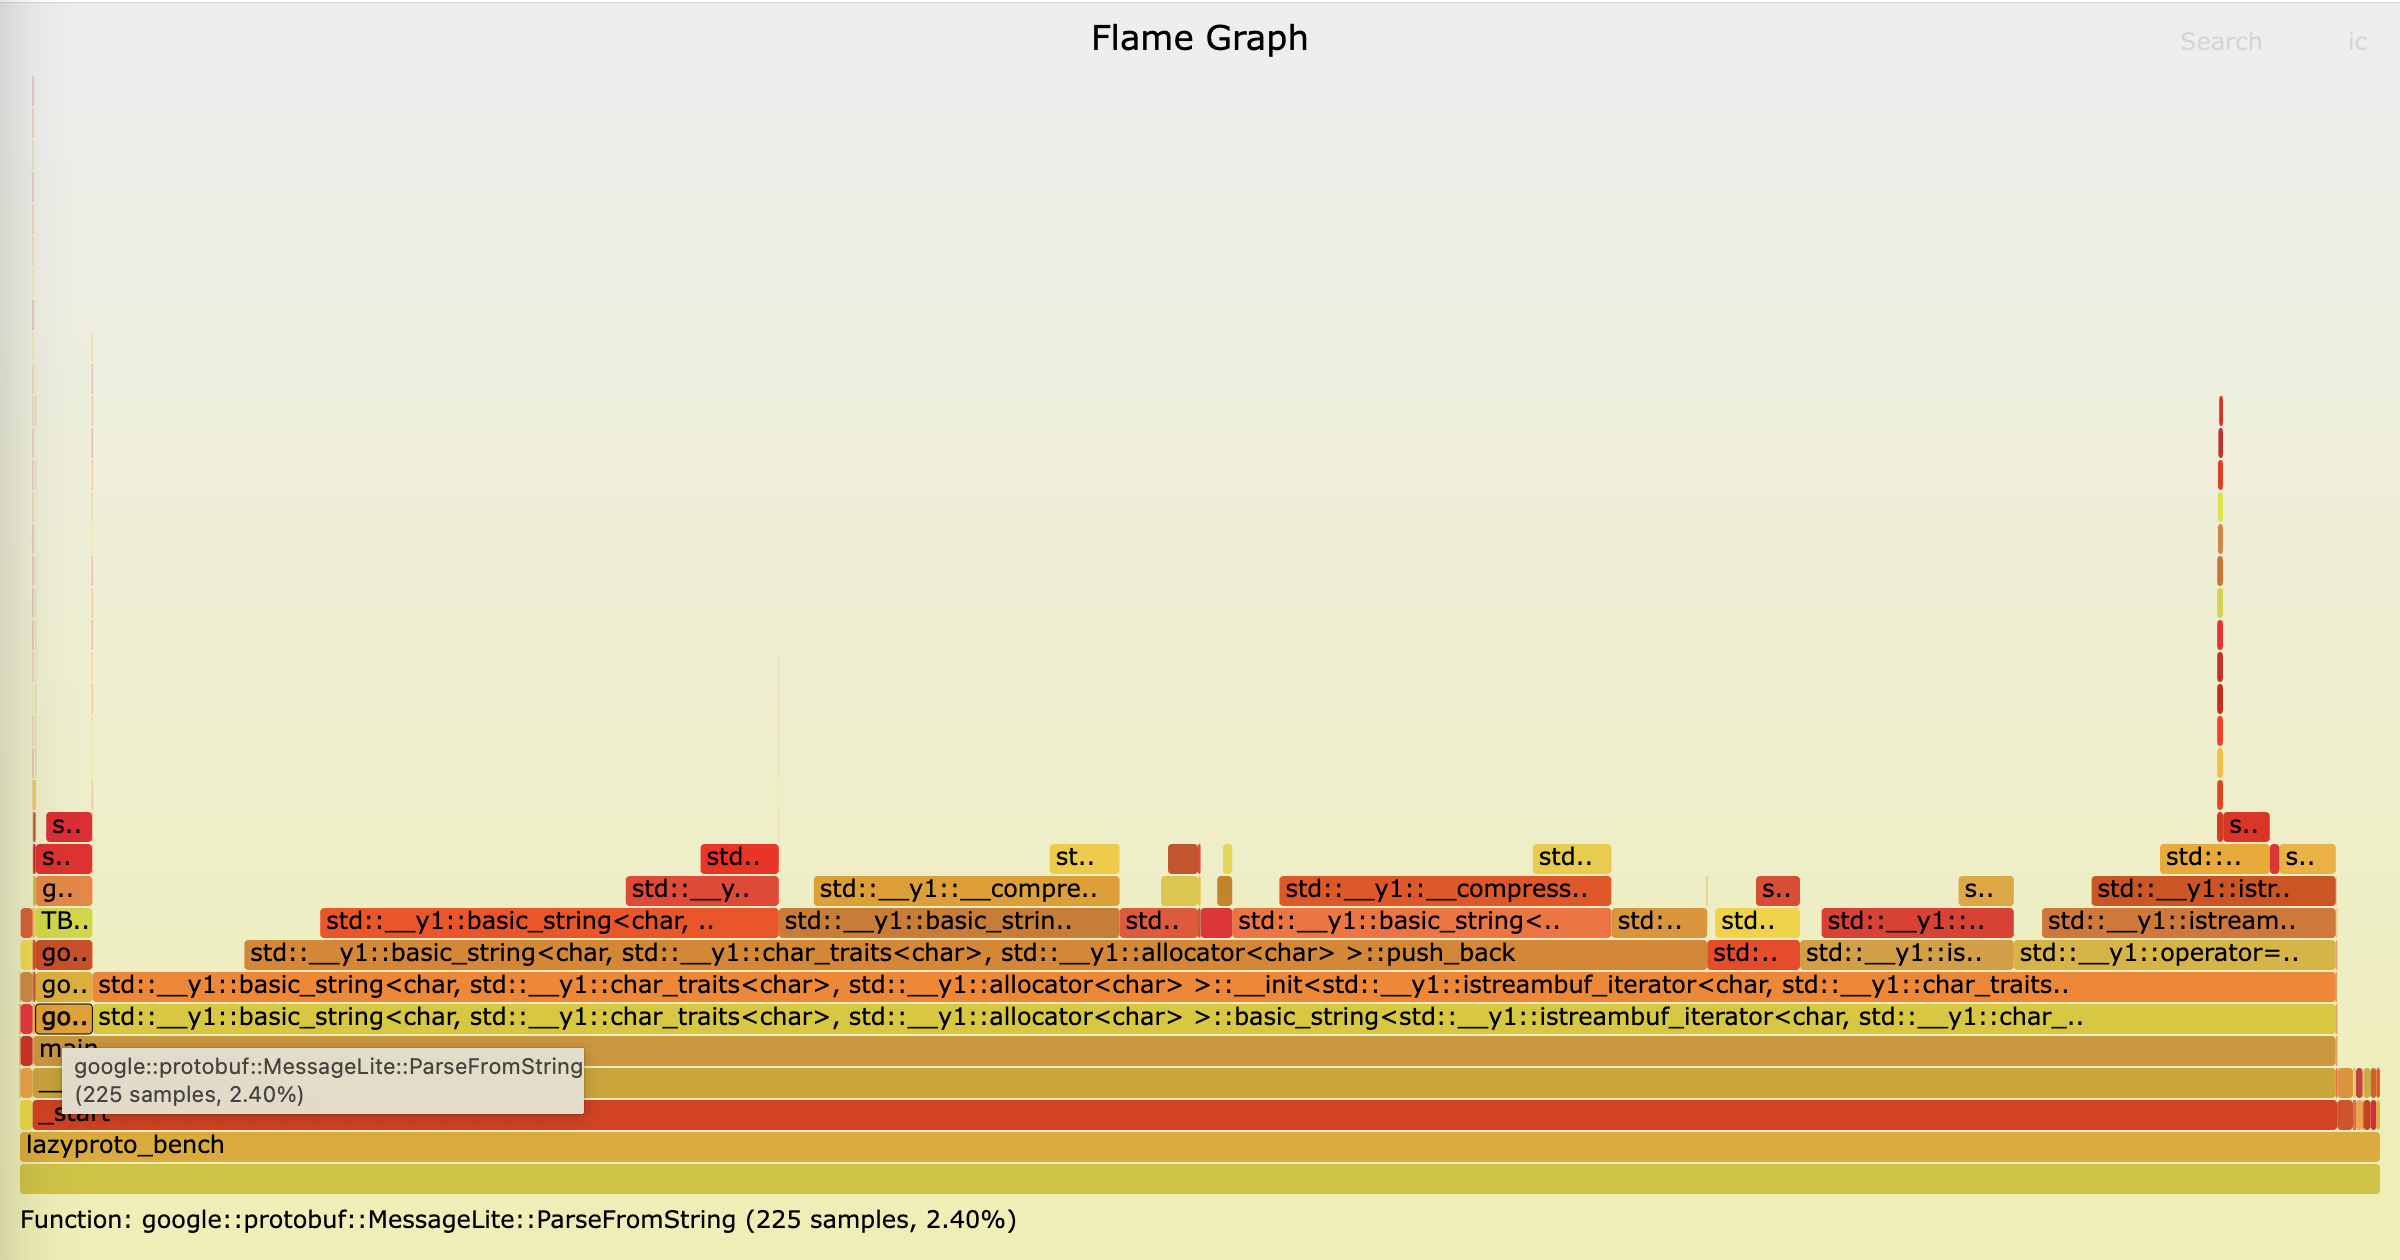
\includegraphics[width=0.70\linewidth]{\commonSecPathPrefix/sec_research_results_attachments/problem1_patched_fgraph.png}
    \caption{Флеймграф алгоритма с изменённым protoc}
    \label{fig:problem1_patched_fgraph}
\end{figure}

Таким образом, для задачи, описанной в подразделе \ref{sec_problem:sec:problem1}, реализованный программный модуль ускоряет работу программы в несколько раз.
На практике величина выигрыша в производительности зависит от процента потока, подходящего под поставленные условия фильтрации, однако даже для большого процента потока
рассмотренная реализация не хуже оригинальной версии компилятора \textit{protoc}.

\subsection{Задача извлечения информации на большом уровне вложенности}

Рассмотрим задачу, описанную в подразделе \ref{sec_problem:sec:problem2}.
В целях замера производительности опишем тестовое protobuf-сообщение, представленное в листинге \ref{sec_research:code:problem2_proto}.

\noindent\begin{minipage}{\linewidth}
\begin{lstlisting}[style=CodeListing, caption={Тестовое protobuf-сообщение}, label=sec_research:code:problem2_proto]
syntax = "proto3";

message TBigProto {
    repeated string StringsArr = 1;
    repeated int32 IntsArr = 2;
    TBigProto BigInternal1 = 3 [lazy_pack = true];
    TBigProto BigInternal2 = 4 [lazy_pack = true];
}
\end{lstlisting}
\end{minipage}

Данное сообщение содержит в себе два поля того же типа, что позволяет создать структуру, напоминающую двоичное дерево из вложенных сообщений типа \textit{TBigProto}.
Таким образом, получится сообщение с большим весом и большой вложенностью.
В листинге \ref{sec_research:code:problem2_build_big_proto} представлена функция \textit{BuildBigInternalMessage}, которая генерирует protobuf-сообщение большого веса на заданном уровне вложенности.

\noindent\begin{minipage}{\linewidth}
\begin{lstlisting}[style=CodeListing, caption={Функция BuildBigInternalMessage}, label=sec_research:code:problem2_build_big_proto]
TBigProto GenBigInternalMessage(
    size_t numOfStrings, size_t lenOfString, size_t numOfInts, size_t level) {
    TBigProto result;
    for (size_t i = 0; i < numOfStrings; i++) {
        result.MutableStringsArr()->Add(GenerateBigString(lenOfString));
    }

    for (size_t i = 0; i < numOfInts; i++) {
        result.MutableIntsArr()->Add(rand() % 500);
    }

    if (level > 0) {
        result.MutableBigInternal1()->CopyFrom(
            GenBigInternalMessage(numOfStrings, lenOfString, numOfInts, level - 1)
        );
        result.MutableBigInternal2()->CopyFrom(
            GenBigInternalMessage(numOfStrings, lenOfString, numOfInts, level - 1)
        );
    }

    return result;
}
\end{lstlisting}
\end{minipage}

В листинге \ref{sec_research:code:problem2_build_test_proto} представлена функция \textit{BuildTestProto}, которая генерирует тестовое protobuf-сообщение с заданным уровнем вложенности, используя функцию \textit{GenBigInternalMessage}.

\noindent\begin{minipage}{\linewidth}
\begin{lstlisting}[style=CodeListing, caption={Функция BuildTestProto}, label=sec_research:code:problem2_build_test_proto]
 void BuildTestProto(size_t numOfStrings, size_t lenOfString, size_t numOfInts) {
     std::ofstream out("./serialized/big_recursive.bin");
     TBigProto bigProto;
     bigProto.CopyFrom(GenBigInternalMessage(numOfStrings, lenOfString, numOfInts, 5));
     out << bigProto.SerializeAsString();
 }
\end{lstlisting}
\end{minipage}

С помощью функции \textit{BuildTestProto} было сгенерировано тестовое сериализованное protobuf-сообщение весом 70 мегабайт.

Рассмотрим функцию для замера производительности \textit{Measure}, представленную в листинге \ref{sec_research:code:problem2_measure}.
Функция читает сериализованное сообщение из файла, парсит его и получает значение на максимальном уровне вложенности.

\noindent\begin{minipage}{\linewidth}
\begin{lstlisting}[style=CodeListing, caption={Функция Measure}, label=sec_research:code:problem2_measure]
void Measure() {
    std::ifstream in("./serialized/big_recursive.bin");
    std::string str(std::istreambuf_iterator<char>{in}, {});
    TString encoded(str);
    TBigProto bigProto;
    Cerr << "---------------\n";
    auto start = TInstant::Now();
    Y_ENSURE(bigProto.ParseFromString(encoded));
    Cerr << "Deserialization took " << (TInstant::Now() - start).MicroSeconds() << "mcs;\n";
    start = TInstant::Now();
    bigProto.GetBigInternal1()
            .Unpack()->GetBigInternal2()
            .Unpack()->GetBigInternal1()
            .Unpack()->GetIntsArr().Get(0);
    Cerr << "Access took " << (TInstant::Now() - start).MicroSeconds() << "mcs\n";
}
\end{lstlisting}
\end{minipage}

На рисунке \ref{fig:problem2_vanilla_timings} представлен замер в случае неизменённого \textit{protoc}.
Десериализация всего сообщения заняла 582 миллисекунды. Стоит отметить, что при перезапусках теста время имеет небольшой разброс.

\begin{figure}[ht]
    \centering
    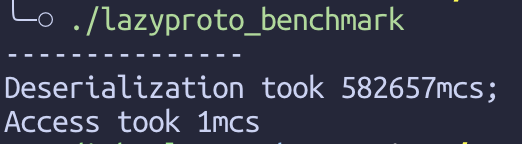
\includegraphics[width=0.70\linewidth]{\commonSecPathPrefix/sec_research_results_attachments/problem2_vanilla_timings.png}
    \caption{Время десериализации сообщения с большой вложенностью в случае неизменённого protoc}
    \label{fig:problem2_vanilla_timings}
\end{figure}

Рассмотрим версию \textit{protoc} с интегрированным модулем <<ленивой>> десериализации.
На рисунке \ref{fig:problem2_patched_timings} представлены результаты замера для той же задачи. Десериализация заняла 218 миллисекунд. Доступ к вложенному полю потребовал 202 миллисекунд. Суммарно десериализация и доступ к полю заняли меньше времени, чем в случае без ленивой десериализации.

\begin{figure}[ht]
    \centering
    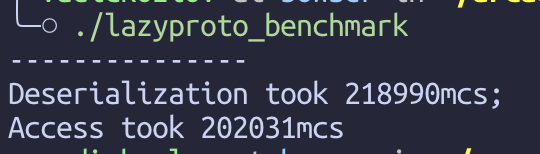
\includegraphics[width=0.70\linewidth]{\commonSecPathPrefix/sec_research_results_attachments/problem2_patched_timings.png}
    \caption{Время десериализации сообщения с большой вложенностью в случае изменённого protoc}
    \label{fig:problem2_patched_timings}
\end{figure}

Построим флеймграфы для данных алгоритмов.
На рисунке \ref{fig:problem2_vanilla_fgraph} представлен флеймграф для алгоритма, использующего неизменённую версию \textit{protoc}. 
Работа с Protocol Buffers занимает 17.5\% от полного времени работы программы.

\begin{figure}[ht]
    \centering
    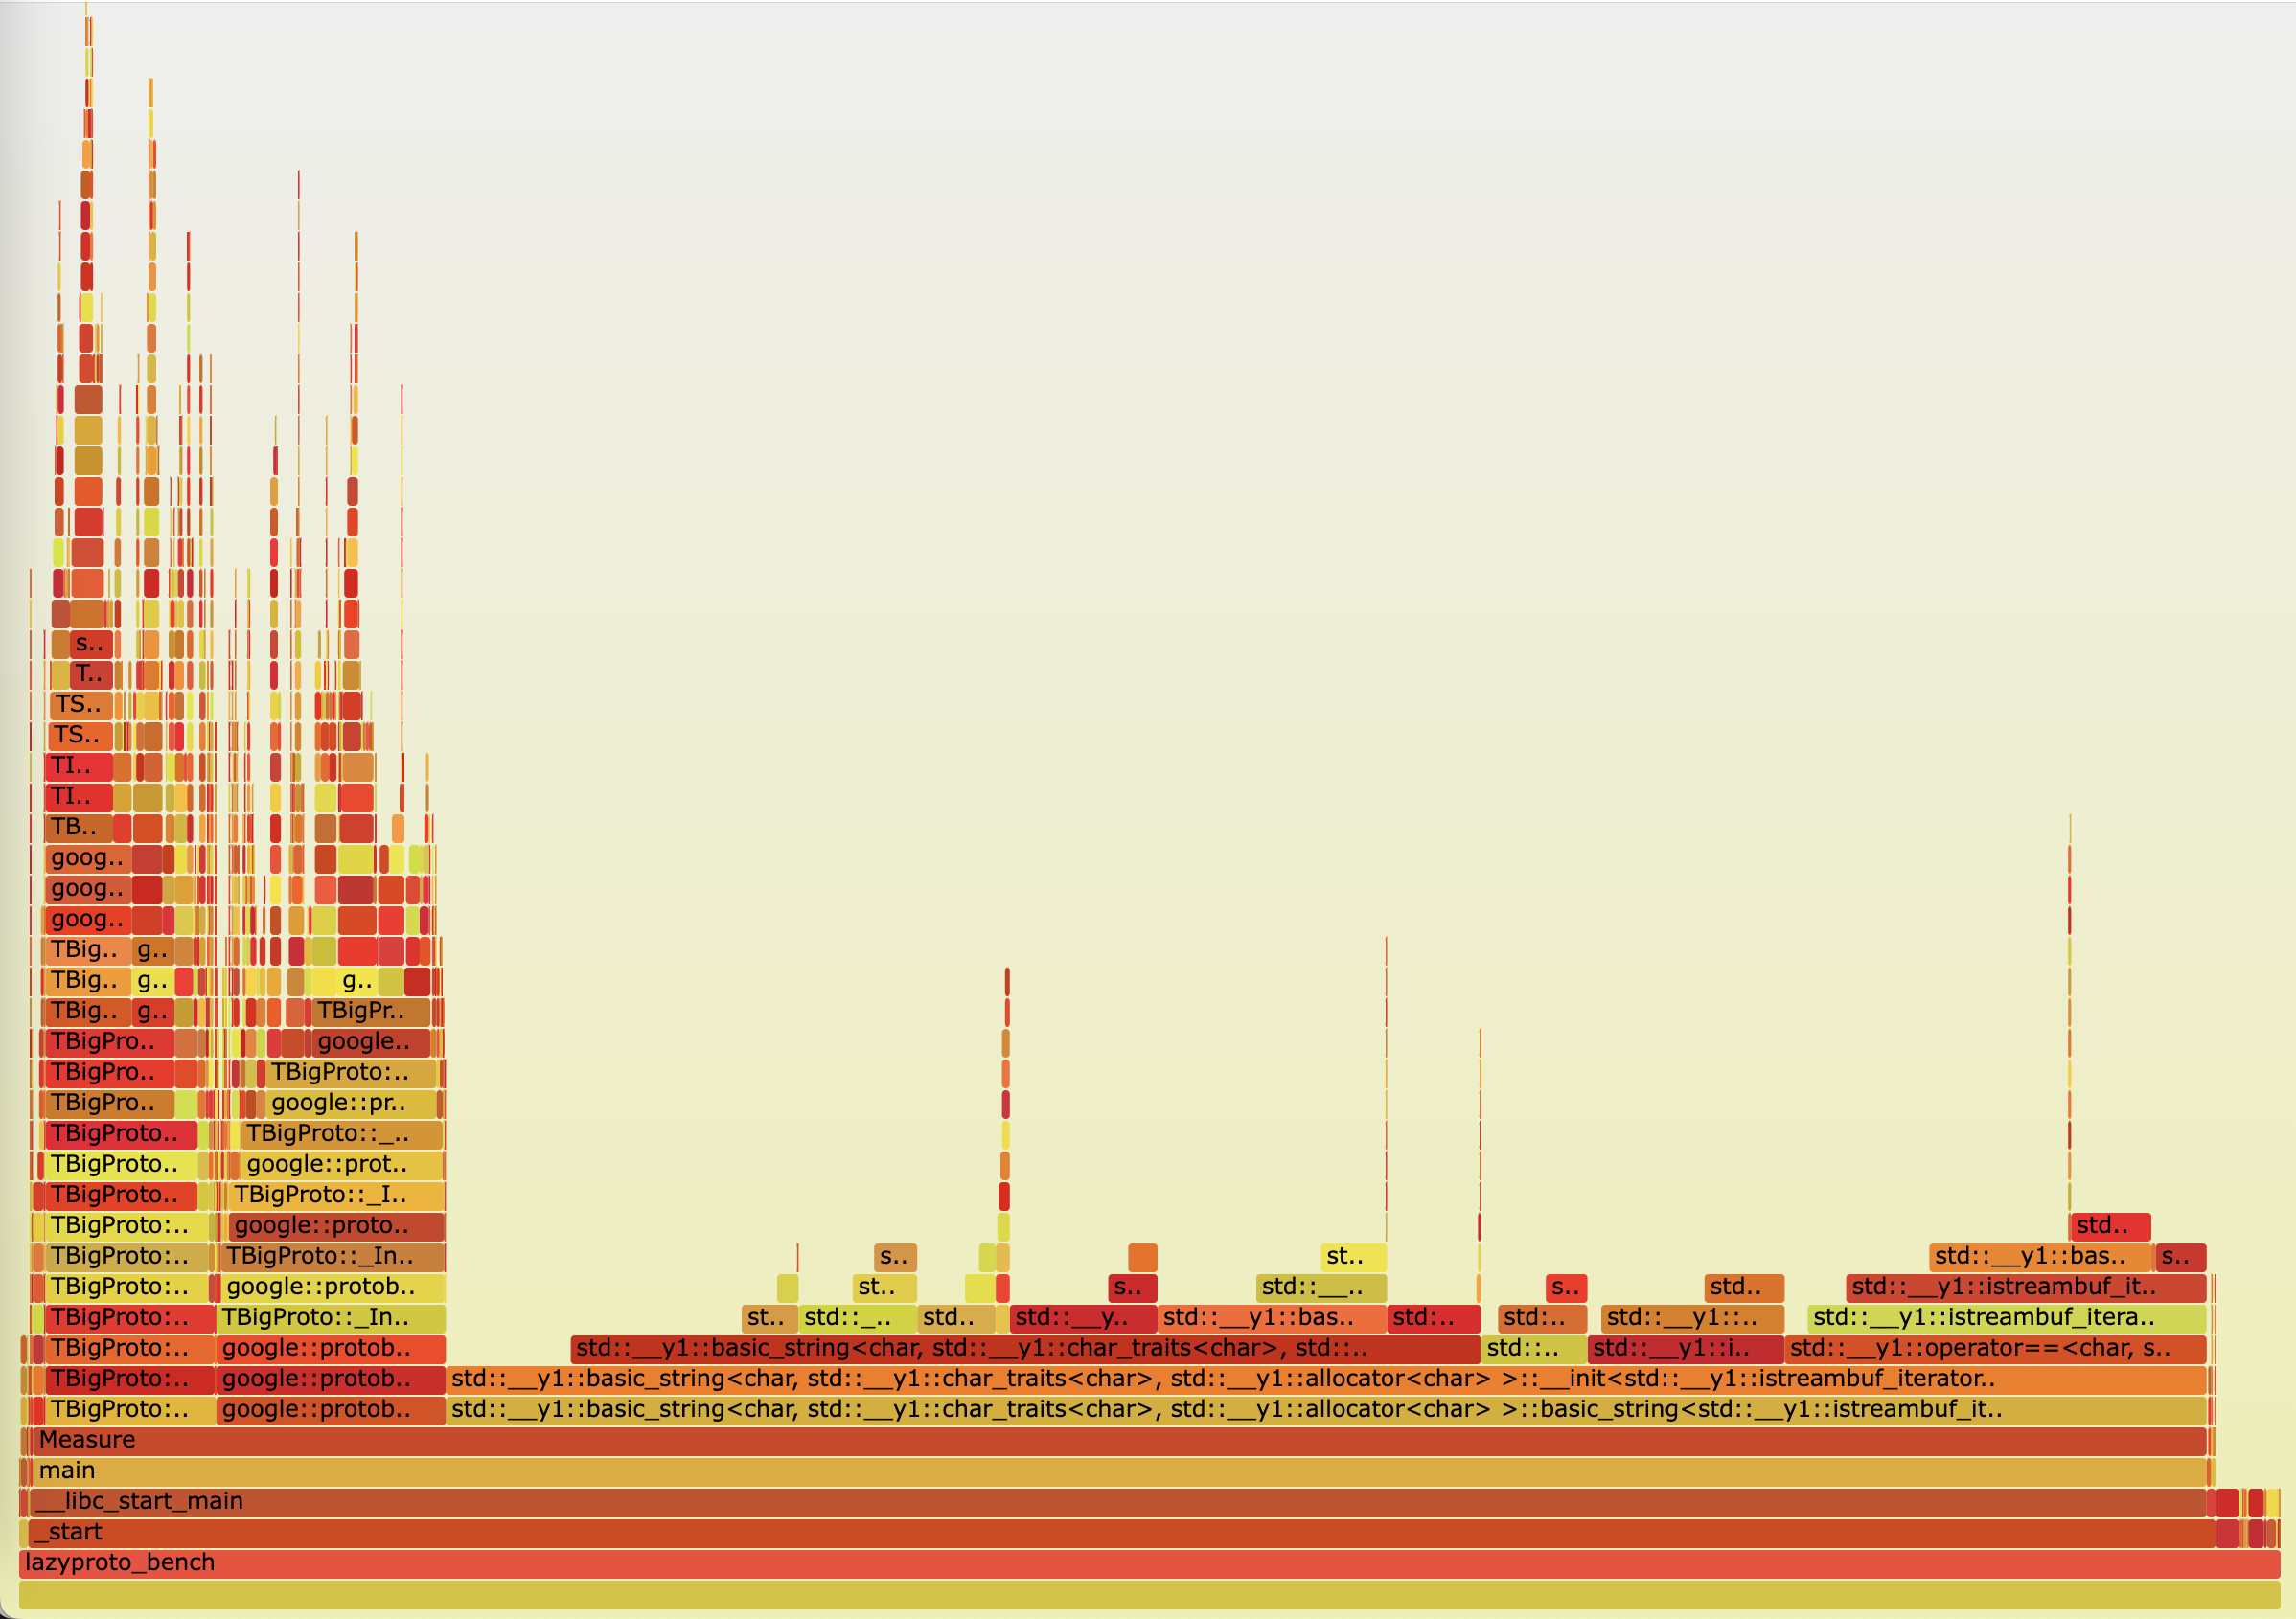
\includegraphics[width=0.70\linewidth]{\commonSecPathPrefix/sec_research_results_attachments/problem2_vanilla_fgraph.png}
    \caption{Флеймграф алгоритма с неизменённым protoc}
    \label{fig:problem2_vanilla_fgraph}
\end{figure}

На рисунке \ref{fig:problem2_patched_fgraph} представлен флеймграф для алгоритма, использующего версию \textit{protoc} с интегрированным модулем <<ленивой>> десериализации. 
Работа с Protocol Buffers занимает 7\% от полного времени работы программы.

\begin{figure}[ht]
    \centering
    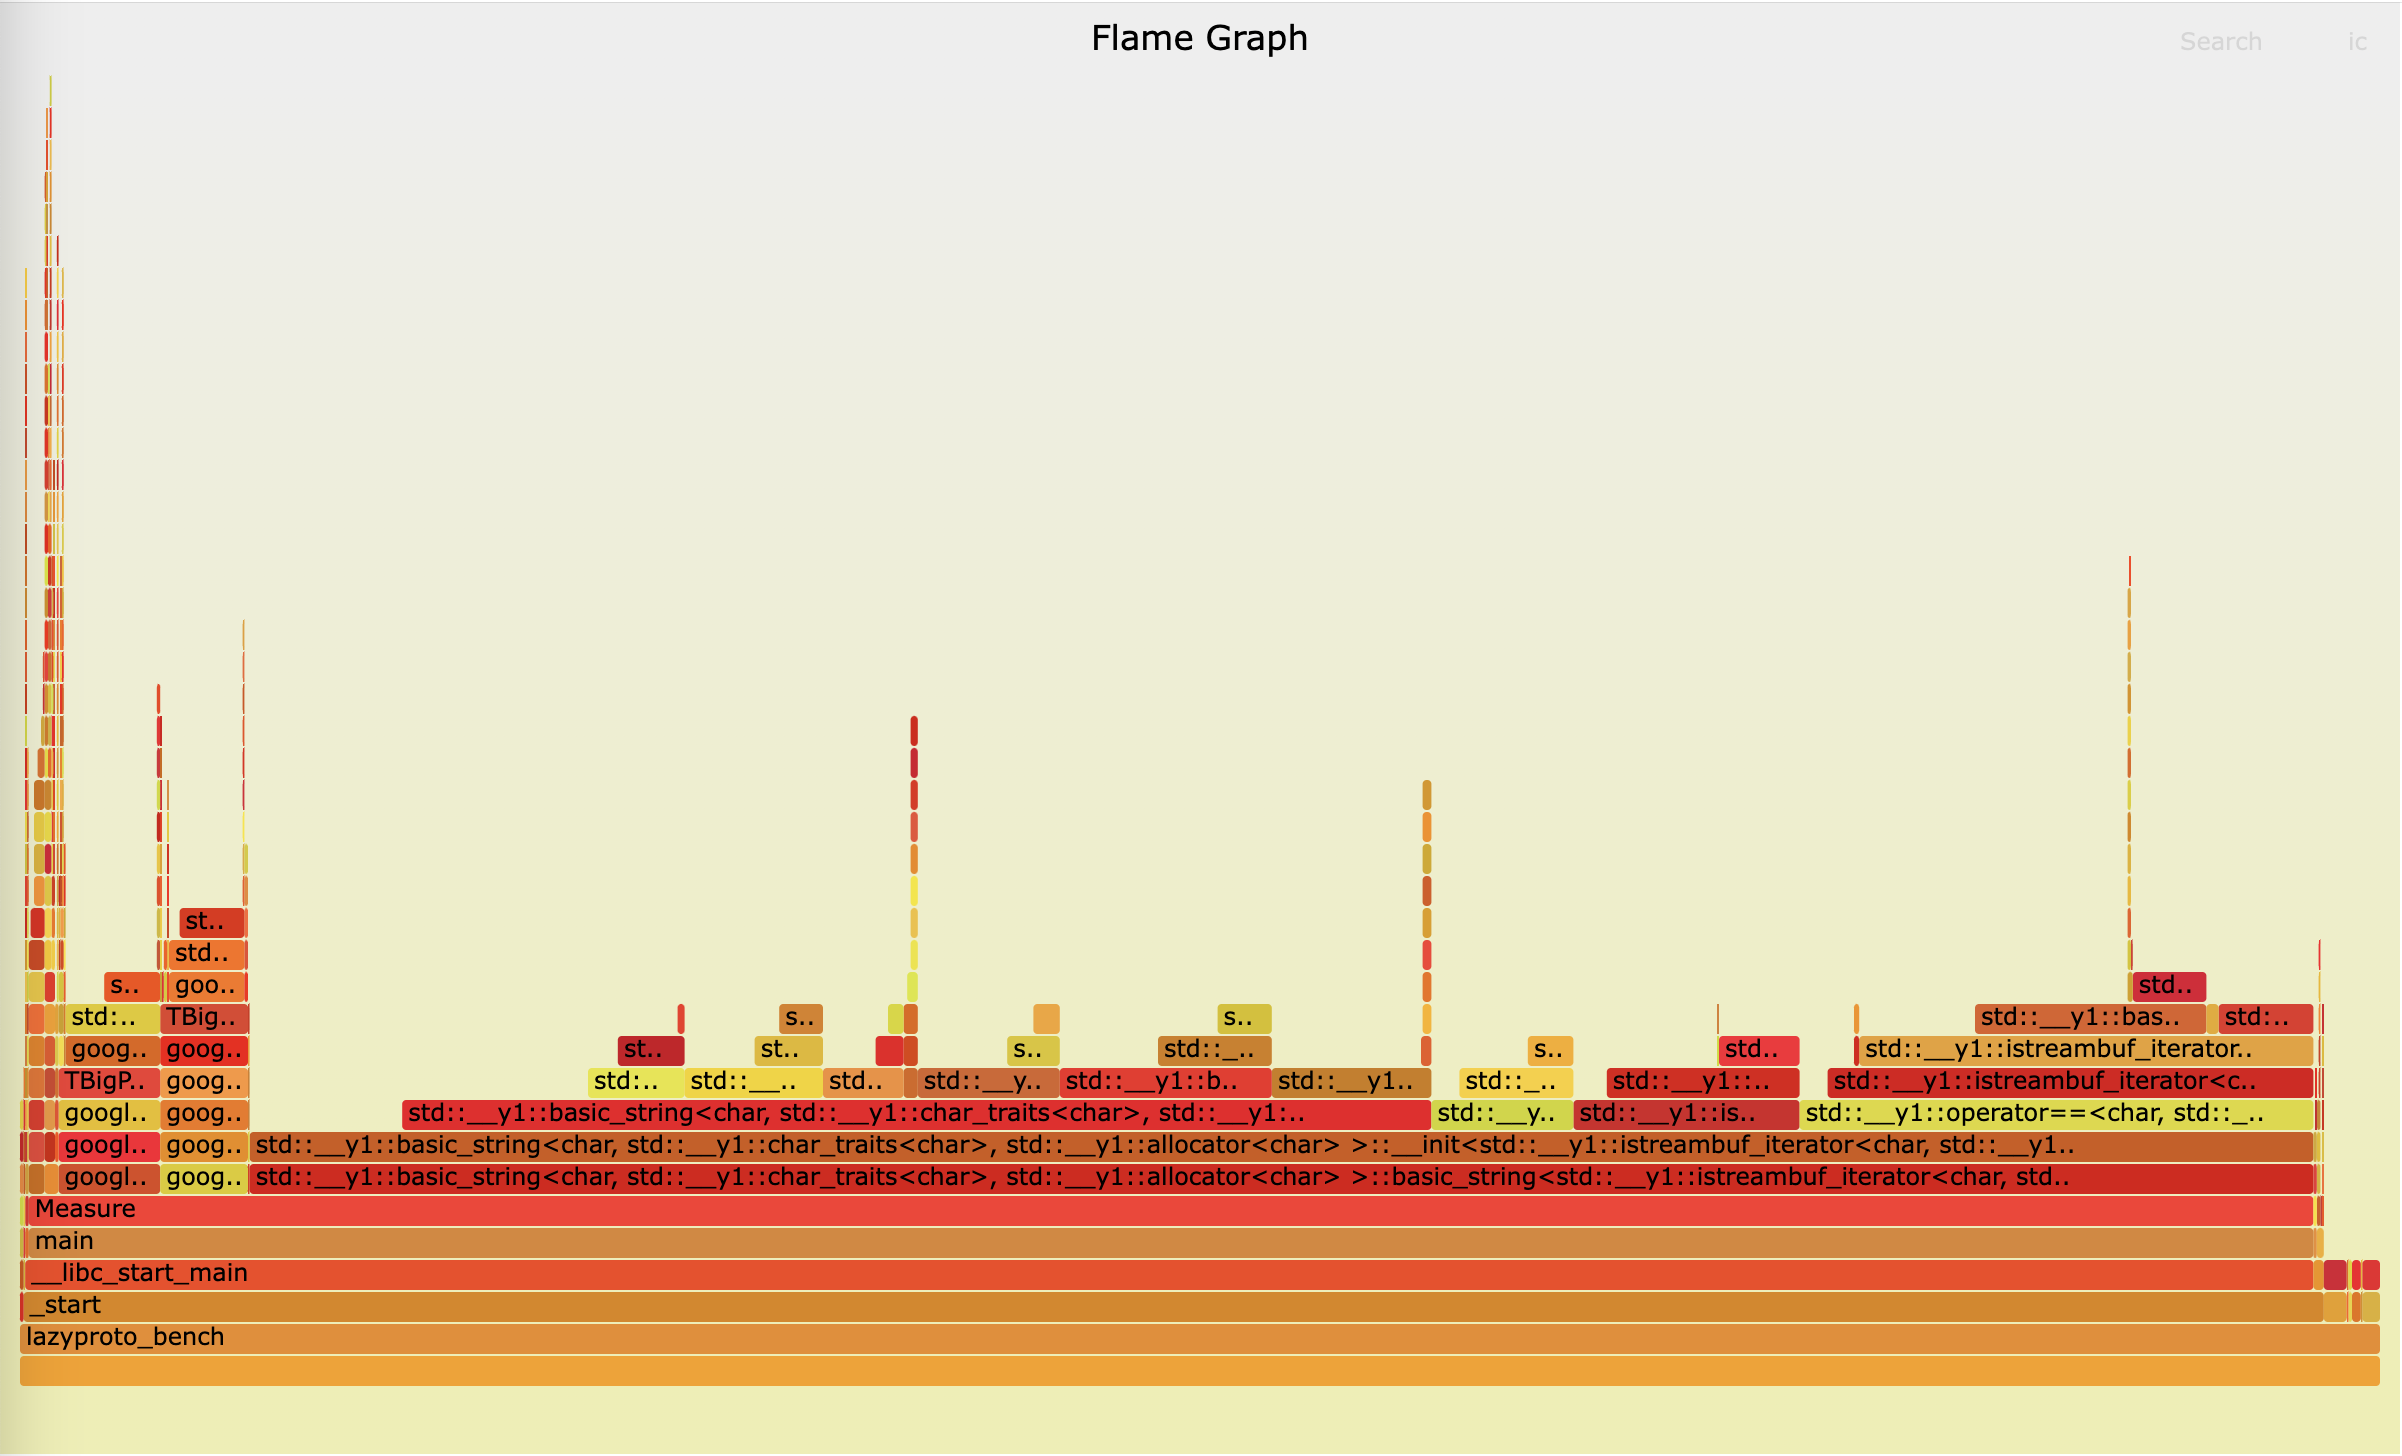
\includegraphics[width=0.70\linewidth]{\commonSecPathPrefix/sec_research_results_attachments/problem2_patched_fgraph.png}
    \caption{Флеймграф алгоритма с изменённым protoc}
    \label{fig:problem2_patched_fgraph}
\end{figure}

Таким образом, предложенная реализация обеспечивает улучшение производительности в задачах, описанных в подразделе \ref{sec_problem:sec:problem2}.
Следовательно даже при смешении обеих рассмотренных задач (фильтрация приходящих сообщений по легковесному полю с большой вложенностью) ожидается выигрыш в производительности.
